\chapter{Implementation}
  In this chapter, we will introduce some specifications of the implementation
  of our solution.\\


  \section{General autocorrelation function}
    The autocorrelation function introduced in Equation \ref{eq:4} can be
    implemented in several ways:

      \subsection{Naive approach}
        The naive approach for the autocorrelation function consists in
        computing all the displacements of the sequence and then
        their correlation with the base sequence as shown in Figure
        \ref{naive_auto:fig:1}. Even though this algorythm is simple and follows
        the mathematical definition, is too slow. We have to compute the
        correlation function for each component leading us to a complexity of
        $O(n^{2})$ where n it the size of the sequence with a huge constant
        as we have to build the shifted sequence for each component.\\

        This constant can be improved if we avoid building the shifts(just
        using slices of the array) but the complexity would stay the same.

      \subsection{Circular convolution theorem}
        [Citation needed]
        The other option is to step in the world of mathematical properties.
        Fortunatly, there exists the convolution theorem that lets us express
        the autocorrelation function in terms of fourier transforms as:
        \begin{theorem}
          Given a sequence $S$ and the Discrete Fourier Transform($DFT$):
          \begin{equation}
            A(S) = DFT^{-1}[DFT\{S\} · DFT\{S\}^{*}]
          \end{equation}
          where $DFT\{S\}^{*}$ represents the complex conjugate of $DFT\{S\}$.
        \end{theorem}

        Notice that, using the Fast Fourier
        Transform\cite{fast_fourier_transform}, the complexity of this
        method lowers to $O(N log N)$. However, it's constant is
        still high as we need to apply 2 FFT to the sequence and apply the
        complex conjugate. In fact we need to keep in mind that Fourier
        Transforms work with complex components while the naive approach keep
        using the same type of components which make it's constant even higher
        than the naive approach.

          \begin{figure}
            \inputpython{Chapters/Implementation/naive.py}{0}{100}
            \caption{An example implementation of the naive autocorrelation}
            \label{naive_auto:fig:1}
          \end{figure}

      \subsection{Specific solution for the composition method}

      If we were to use a general method for this computation, we would probably
      use the one based in Fourier Transforms because we will be dealing with
      long sequences that will compensate the big constant of this method.\\

      However, we are dealing with sequences with the special property of
      having been built through the composition method. This means that we
      might find a non general way of computing this autocorrelation with better
      computational characteristics.\\

      If we take advantage of property \ref{composition:prop:1}, we can design
      an algortytm with interesting properties. First of all, the complexity
      function depends on the size of the shift sequence. Being $m$ the
      length of the shift sequence and $n$ the length of the composite
      sequence, the resulting algortyhm has a complexity of $O(nm)$. This means
      that when $m < log(n)$ this algorythm has a better complexity than the
      Fourier Transform's approach.\\

      In addition, this algorythm has a better constant. We just need to
      iterate once through the autocorrelation sequence, it's more cache
      friendly as the data source of the function is smaller and it doesn't
      need to use complex operations in binary sequences.\\

      But the biggest improvement in respect of the fourier transform is that
      the complexity of a partial result of size $p$ is $O(mp)$ while the
      convolution theorem requires $O(nlog(n))$ for a partial result. In
      practice this means that if we just want to check a certain property
      of the autocorrelation we have no need to compute the whole function.\\

      An example implementation of this algorythm is shown in Figure \ref{composite_auto:fig:1}

      \begin{figure}[ht!]
        \inputpython{Chapters/Implementation/composite.py}{0}{100}
        \caption{A pure python implementation to illustrate the algorythm. In
        the software project it's implemented in Cython}
        \label{composite_auto:fig:1}
      \end{figure}

  \section{Search space}

  Given a base sequence of size $n$ and a length $m$ for the shift sequences,
  our program needs to find all the shift sequences that generate a composite
  sequence with a good autocorrelation.\\

  This means that the search space are all the posible permutations of the
  shift sequence, in other words, $n^m$ permutations. However, there are some
  relations between the different shift sequences that let us narrow the
  search space.\\

  For example, if we add a constant to every component to the shift sequence,
  we get a shifted version of the same sequence. This means that if we only
  computed the permutations that start with the same component, we would cover
  the whole search space as any other permutations would be just shifts of
  a one permutation from the computed set. This optimization narrows our
  search space to $n^{(m-1)}$\\

  Other optimization arises from the form of the shift sequences. In general,
  if the symbols are repeated often, they trend to generate higher
  autocorrelation spikes or periods inside the composite sequence. This
  concept can be easily with the Hamming autocorrelation function:\\

  \begin{definition}[Hamming autocorrelation]
    Given a sequence $S$ of length $n$ and the function $shift$ defined at
    Equation \ref{eq:3}, we define the Hamming autocorrealtion as:
      \begin{equation}
        HA(S)_{\ŧau} = \sum_{i=0}^{n} HAComponent(S_{\tau}, shift(S, \tau)_{\tau})
      \end{equation}
    where $HAComponent$ is defined as:
      \begin{equation}
        HAComponent(c1, c2) = \left\{\begin{array}{lr}
            1  &  c1 = c2\\
            0  & \textnormal{otherwise} \\
        \end{array}\right.
      \end{equation}
  \end{definition}

  For our branch and bound algorythm, it's important to note that if we
  substitute a symbol that only appears one for another, the hamming
  autocorrelation won't get lower. This means that if we do a depth-in first
  bounding the nodes that have a hamming autocorrelation higher than the
  threshold(we mean, the maximum non trivial component) we are sure that all
  that branch have a higher hamming autocorrelation than the threshold.\\

  \begin{figure}[ht!]
    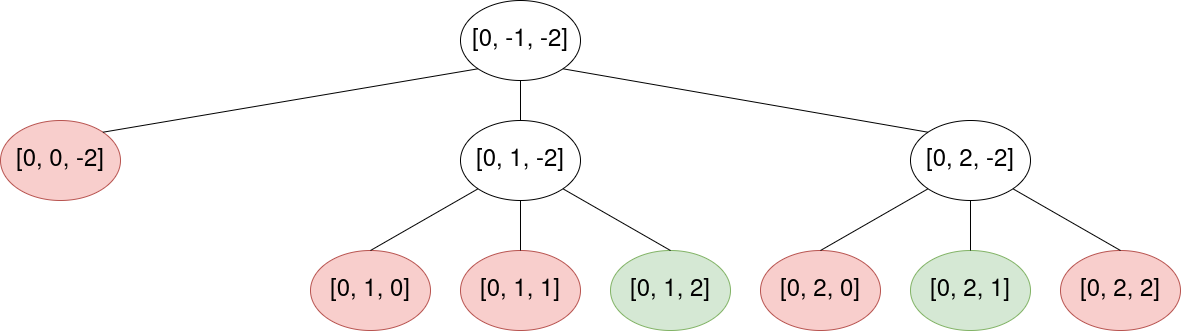
\includegraphics[scale=0.4]{Chapters/Implementation/Example_branch_bound.png}
    \caption{An example of the branch and bound algorythm with a threshold for hamming autocorrelation of 1 and a base sequence of length 3. Red nodes represent boundings and green ones final nodes in which the autocorrelation is computed and checked. Negative values represent values that haven't been initialized yet.}
    \label{bb:fig:1}
  \end{figure}

  We can deduce several thing from Figure \ref{bb:fig:1}:
  \begin{itemize}
    \item we reduce the number of autocorrelations computed by a significant amount
    \item The computation on each branch isn't balanced. This must be taken into account when we desing the parallelism model
  \end{itemize}

  \section{Parallelism model}
